\section{Navigating the Design and User Experience of our Python GUI}

Throughout our project, a key aspect of our development journey involved creating a straightforward Python GUI program. This application empowers users to effortlessly experiment with various models and seamlessly obtain insightful visualizations of hypergraphs. Additionally, users can leverage the GUI to benchmark different models, providing a user-friendly interface for comprehensive exploration.

\noindent\hrulefill

\textbf{Features at a Glance:}

\begin{description}
    \item[Model Trial:] Easily try out different models with a user-friendly interface, allowing for quick experimentation and comparison.
    \item[Hypergraph Visualization:] Gain valuable insights through simple visualizations of hypergraphs, providing a clear representation of complex structures.
    \item[Benchmarking Capabilities:] Evaluate model performance efficiently by benchmarking against diverse datasets, aiding in the assessment and selection of the most suitable models.
\end{description}

\noindent\hrulefill    

In the following sections, we will delve into the design principles and functionalities of our Python GUI, offering guidance on its usage and showcasing its potential for enhancing your modeling experience.

\subsection{  Installing and Running the GUI}

To kickstart your exploration of oriented hypergraphs with our Python GUI, follow these simple steps to install and run the program:

\textbf{Step 1: Get the Code}

Visit our GitHub repository at \url{https://github.com/ZephyrSV/tfg_python/} and clone or download the code to your local machine.

\textbf{Step 2: Install python}

Ensure that you have Python installed on your system. If not, download and install it from the official Python website: \url{https://www.python.org/downloads/}

\textbf{Step 3: Install AMPL}

Make sure you have at least the free community version of AMPL installed on your device. You can download it from the AMPL website: \url{https://ampl.com/products/solvers/free-software/}

\textbf{Step 4: Set up the virtual environment}
Next, create a virtual environment (venv) to isolate dependencies for the GUI. Open your terminal or command prompt and navigate to the directory containing the program files. Execute the following commands:

\begin{verbatim}
# Create a virtual environment
python -m venv venv

# Activate the virtual environment
# On Windows
venv\Scripts\activate
# On Unix or MacOS
source venv/bin/activate
\end{verbatim}

This creates and activates the virtual environment. Note: Depending on your terminal app, you may need to use a different activation script (e.g., `activate.ps1` on Windows Powershell).

\textbf{Step 5: Install Dependencies}

While the virtual environment is active, install the required libraries using the following command:

\begin{verbatim}
pip install -r requirements.txt
\end{verbatim}

This command installs the necessary dependencies for the GUI within the virtual environment.


\textbf{Step 6: Run the GUI}

With the virtual environment still active and AMPL installed, navigate to the directory containing the program files and run the following command:

\begin{verbatim}
python3 App.py
\end{verbatim}

This command launches the Python GUI application.

\subsection{Pathway Selector}

The "Pathway Selector" serves as the central hub for navigating and interacting with our program.

Below, we show 2 screenshots. \\
The first one (Figure \ref{fig:pathway_selector}) is of the main page as it is shown to the user. \\
The second (Figure \ref{fig:pathway_selector_labeled_features}) shows the same image except that we have included labels for each feature present on the main page. We will then refer to these labels in the rest of the section.

\begin{figure}[H]
    \centering
    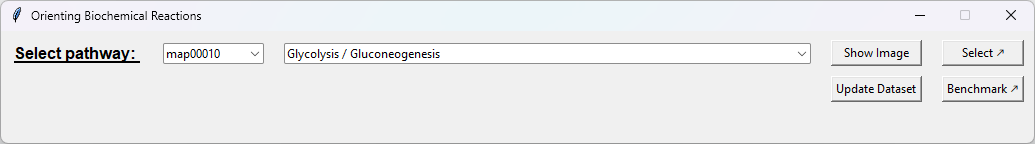
\includegraphics[width=0.8\textwidth]{Design of the User Interface/selector.png}
    \caption{Pathway Selector - User view}
    \label{fig:pathway_selector}
\end{figure}

\begin{figure}[H]
    \centering
    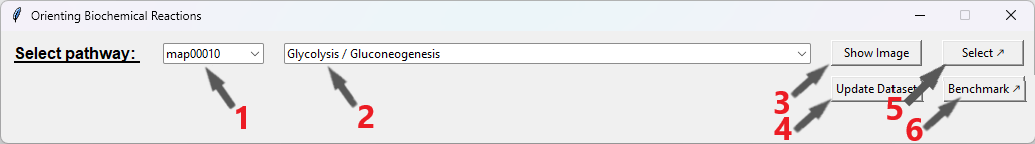
\includegraphics[width=0.8\textwidth]{Design of the User Interface/selector labeled.png}
    \caption{Pathway Selector - Labeled Features}
    \label{fig:pathway_selector_labeled_features}
\end{figure}
Let's explore the features available on this main page:

\textbf{Pathway Selection Options:}

\begin{enumerate}
    \item \textbf{Select by ID:} Utilize the dropdown menu to choose a pathway based on its unique identifier (ID). The user can also type in a search string in the field and pressing enter. The dropdown will then filter out all entries that do not contain the search string.
    \item \textbf{Select by Description:} Alternatively, you can opt for pathway selection by choosing a human-readable description from the dropdown menu. In the same way as before, the user 
\end{enumerate}


\textbf{Buttons and Actions:}

\begin{enumerate} 
\setcounter{enumi}{2}   

    \item \textbf{Show Image:} Clicking this button will fetch and display the image of the selected pathway from the KEGG database, providing a visual representation of its structure. See Figure \ref{fig:show_image} for an example.

    \item \textbf{Update Dataset:} This button allows the user to rebuild the dataset used to create the models of the pathways.
    
    \item \textbf{Select:} Access the solver/visualizer tool by clicking this button, enabling in-depth exploration and analysis of the chosen pathway.
    
    \item \textbf{Benchmark:} Evaluate and compare model performances on 25 models, facilitating comprehensive assessments.
\end{enumerate}

\begin{figure}[H]
    \centering
    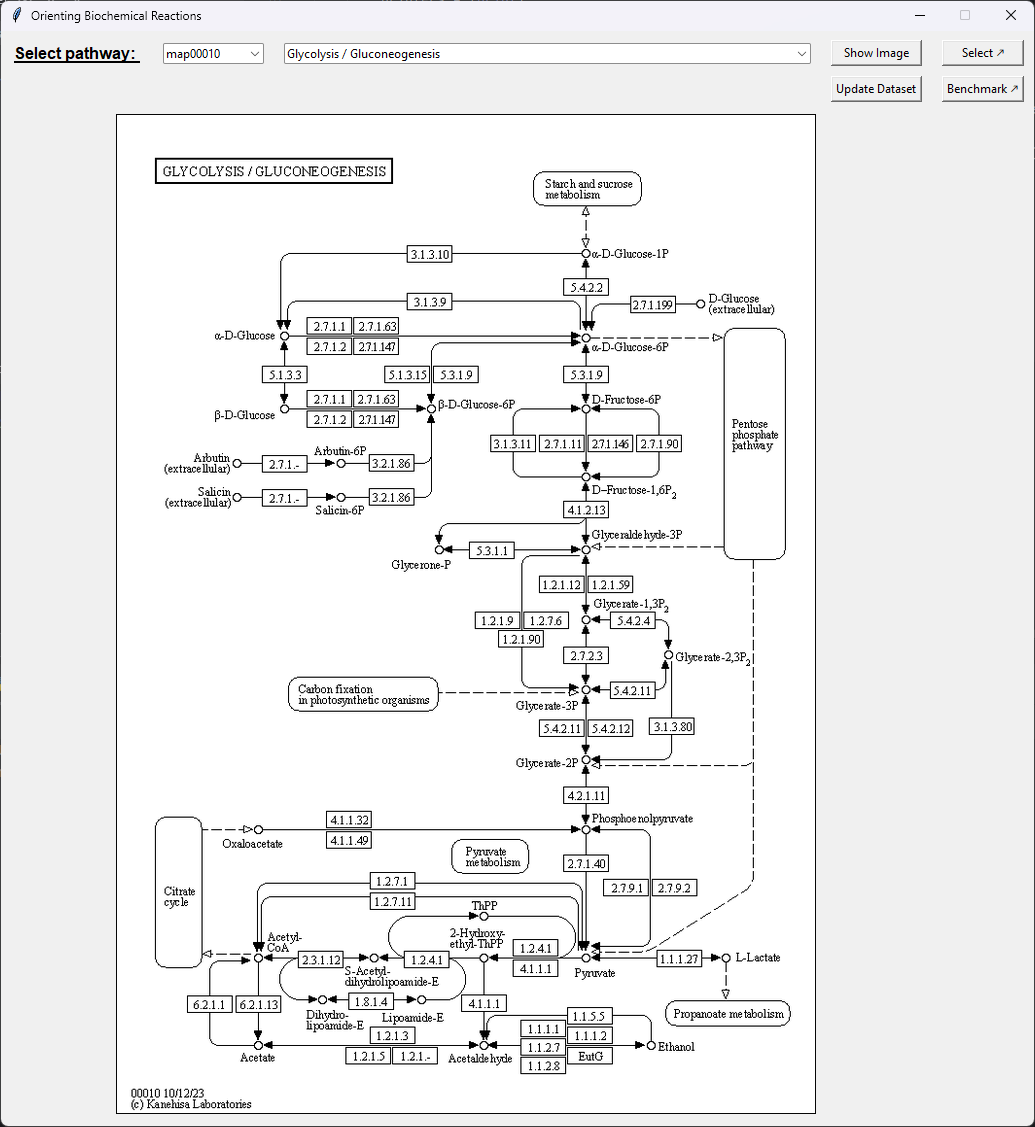
\includegraphics[width=0.8\textwidth]{Design of the User Interface/image_pathway.png}
    \caption{Show Image - Image corresponding to the entry 'map00010'}
    \label{fig:show_image}
\end{figure}

\textbf{Note:} Tooltips are available for each feature. Hover your mouse over any feature to view a brief explanation of its functionality. View Figure \ref{fig:show_image_tooltip} for an example.

\begin{figure}[H]
    \centering
    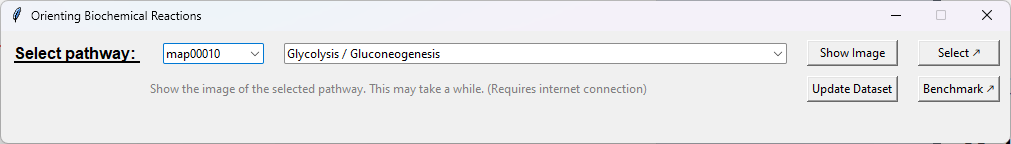
\includegraphics[width=0.8\textwidth]{Design of the User Interface/tip_show_image.png}
    \caption{Feature tooltips - tooltip of the show image button}
    \label{fig:show_image_tooltip}
\end{figure}

Upon pressing the \textbf{Update Dataset} button, a crucial warning message promptly emerges to alert the user about the potential duration of the operation, as depicted in Figure \ref{fig:update_warning}.

\begin{figure} [H]
\centering
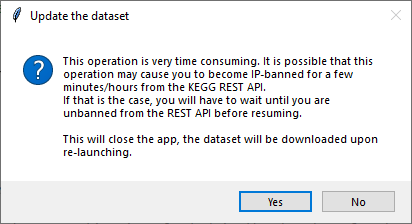
\includegraphics[width=0.5\linewidth]{Design of the User Interface/update_warning.png}
\caption{Warning Message on Updating Dataset}
\label{fig:update_warning}
\end{figure}

The warning message reads as follows:

\begin{quote}
\textit{This operation is very time-consuming. It is possible that this operation may cause you to become IP-banned for a few minutes/hours from the KEGG REST API.\
If that is the case, you will have to wait until you are unbanned from the REST API before resuming.\\
\\
This will close the app, and the dataset will be downloaded upon re-launching."}
\end{quote}

This cautionary message aims to ensure that users are fully aware of the potential consequences and the time commitment associated with updating the dataset. It emphasizes the possibility of temporary IP-banning and provides guidance on the necessary steps if such an event occurs.

\subsection{Pathway Solver/Visualizer}

The "Solver/Visualizer" view provides a comprehensive environment for in-depth exploration and analysis of the selected pathway. This view offers tools and features that empower users to interact with the oriented hypergraph representation and derive meaningful insights. 

\begin{figure}[H]
    \centering
    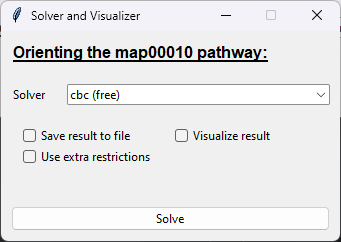
\includegraphics{Design of the User Interface/solver_visualizer.png}
    \caption{Solver/Visualizer - User View}
    \label{fig:solver_visualizer}
\end{figure}

Let's delve into the key components and functionalities of this view:
\begin{itemize}
    \item \textbf{Solver Selection Dropdown:} Users can choose from a dropdown menu to select the solver they want to use (CBC, Gurobi or CPLEX).\footnote{\textbf{Note:} CBC is marked as free, as you don't need a licence to use it. Unlike Gurobi and CPLEX.}
    \item \textbf{Save to File Tickbox:} A tickbox allowing users to specify whether to save the solver results to a file.
    \item \textbf{Visualize Result Tickbox:} Users can choose to visualize the solver results by ticking this option.
    \item \textbf{Use Extra Restrictions Tickbox:} This tickbox enables users to apply additional restrictions to the solver process if needed.
    \item \textbf{Solve Button:} The SOLVE button triggers the solving of the AMPL problem with the chosen solver and configurations.
\end{itemize}

Upon pressing the \textbf{Solve} button, a new instance of AMPL is created, the model and the pathway are loaded and after setting the solver, the optimization problem is completed. 

The ensuing Figure \ref{fig:output-map00908} illustrates the output presentation:

\begin{figure}[H]
    \centering
    \begin{framed}
    \begin{small}
    \begin{verbatim}
###############################################
### Computed in 0.1814289093017578 seconds
### Number of internal vertices  28
###############################################

### reactionID : [Substrates] : [Products]

### Reactions that were not inverted
R01122 : C00235 C17324 : C00013 C04432
R02119 : C00190 C00371 : C00015 C03300
R03133 : C00979 C00371 : C01513 C00033
R03726 : C00019 C04083 : C00170 C01804
R04038 : C00235 C00020 : C00013 C04713
R05708 : C04083 C00001 C00028 : C00147 C07330 C00030
R07260 : C00029 C15545 : C00015 C15546
R08051 : C00235 C00002 : C16424 C00013
R08053 : C16424 C03024 C00007 : C16428 C03161 C00001
R08054 : C16426 C03024 C00007 : C16429 C03161 C00001
R08055 : C04713 C03024 C00007 : C16430 C03161 C00001
R08061 : C16424 C00001 : C16426 C00009
R08062 : C16426 C00001 : C04713 C00009
R08063 : C16428 C00001 : C16429 C00009
R08064 : C16429 C00001 : C16430 C00009
R08065 : C16430 : C16445
R08066 : C16427 C03024 C00007 : C16431 C03161 C00001
R08067 : C16431 : C16447
R08070 : C16430 C00001 : C16431 C00009
R08071 : C16445 C00001 : C16447 C00009
R08073 : C16431 C00001 : C00371 C00121
R08074 : C16447 C00001 : C02029 C00121
R08075 : C00371 C00029 : C16443 C00015
R08076 : C02029 C00029 : C16448 C00015
R08077 : C04432 : C16467
R08078 : C16467 : C16441
R08079 : C16441 C00001 : C16449 C00009
R08080 : C16449 C00001 : C15545 C00121
### Reactions that were inverted
R02118 : C00015 C03423 : C00029 C00371
R05702 : C00371 C00005 C00080 : C02029 C00006
R08052 : C16426 C00013 : C00235 C00008
R08068 : C00371 C03161 C00001 : C04083 C03024 C00007
R08069 : C16427 C00009 : C04713 C00001
R08072 : C04083 C00121 : C16427 C00001
    \end{verbatim}
    \end{small}
    \end{framed}
    \caption{Output for map00908 - Zeatin biosynthesis}
    \label{fig:output-map00908}
\end{figure}

By default, the output is directed to the console. However, when the \textbf{Save to file} tickbox is selected, the program prompts the user to designate a location for saving the output, as depicted in Figure \ref{fig:save-as}.

\begin{figure}[H]
    \centering
    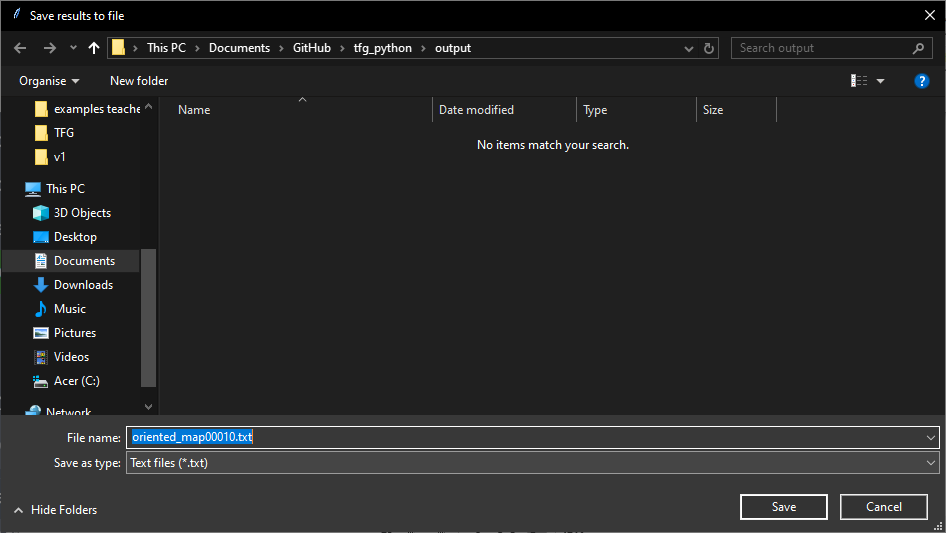
\includegraphics[width=0.8\textwidth]{Design of the User Interface/save-as.png}
    \caption{Solver-Visualizer - Saving the result in a file}
    \label{fig:save-as}
\end{figure}

f the user opts for the \textbf{Visualize results} tickbox, a representation of the model, generated using the Python library \href{https://networkx.org/}{networkx} is presented. This representation utilizes a graph to depict our hypergraph. The transformation from a hypergraph to a graph is achieved through the following mathematical procedure:

\begin{framed}
\begin{procedure} Representing a hypergraph using a graph.

Given an hypergraph H = (V, E), where V is the set of \textbf{vertices} and E of \textbf{hyperedges}, 
we create the graph G = ($V~\bigcup~E$, $E_T~\bigcup~E_H$), where:
\begin{align*}
    &E_T = \{\{u,~\{T,~H\}\}~\mid~u~\in~V,~\{T,~H\}~\in~E,~u~\in~T\}\\
    &E_H = \{\{u,~\{T,~H\}\}~\mid~u~\in~V,~\{T,~H\}~\in~E,~u~\in~H\} 
\end{align*}
We give an example of applying this procedure in Figure \ref{fig:hypergraph_as_graph}.

\begin{figure}[H]
    \centering
    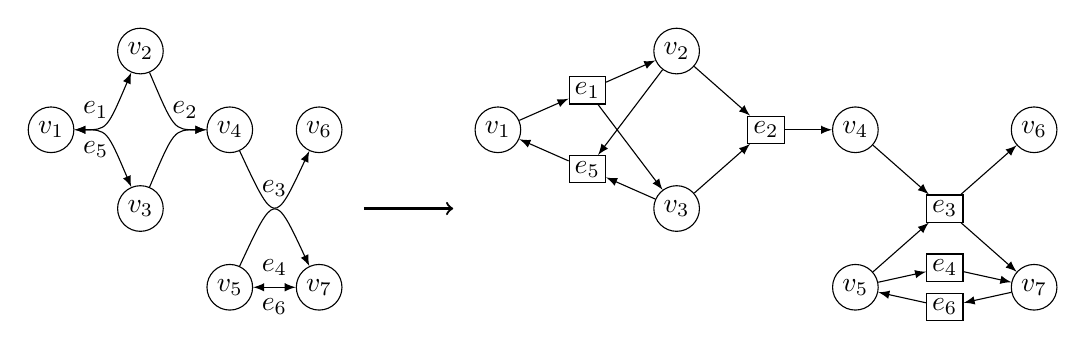
\begin{tikzpicture}[baseline,xscale=0.5675]
    \tikzstyle{every picture}=[thick]
    \tikzstyle{every node}=[inner sep=2pt,circle,draw]
    \draw (0,2) node (1) {$v_1$};
    \draw (2,3) node (2) {$v_2$};
    \draw (2,1) node (3) {$v_3$};
    \draw (4,2) node (4) {$v_4$};
    \draw (4,0) node (5) {$v_5$};
    \draw (6,2) node (6) {$v_6$};
    \draw (6,0) node (7) {$v_7$};
    \draw[latex-latex] (1) .. controls (1.25,2) .. (2);
    \draw[latex-latex] (1) .. controls (1.25,2) .. (3);
    \draw[-latex] (2) .. controls (2.75,2) .. (4);
    \draw[-latex] (3) .. controls (2.75,2) .. (4);
    \draw[-latex] (4) .. controls (5,0.78125) .. (6);
    \draw[-latex] (5) .. controls (5,1.21875) .. (7);
    \draw[latex-latex] (5) -- (7);
    \draw (1,2.25) node[draw=none] {$e_1$};
    \draw (3,2.25) node[draw=none] {$e_2$};
    \draw (5,1.25) node[draw=none] {$e_3$};
    \draw (5,0.25) node[draw=none] {$e_4$};
    \draw (1,1.75) node[draw=none] {$e_5$};
    \draw (5,-0.25) node[draw=none] {$e_6$};
    %%%%%
    \draw[->, thick] (7,1) -- (9,1);
    %%%%
    \draw (10,2) node (1) {$v_1$};
    \draw (14,3) node (2) {$v_2$};
    \draw (14,1) node (3) {$v_3$};
    \draw (18,2) node (4) {$v_4$};
    \draw (18,0) node (5) {$v_5$};
    \draw (22,2) node (6) {$v_6$};
    \draw (22,0) node (7) {$v_7$};
    \draw (12,2.5) node[rectangle] (8) {$e_1$};
    \draw (16,2) node[rectangle] (9) {$e_2$};
    \draw (20,1) node[rectangle] (10) {$e_3$};
    \draw (20,0.25) node[rectangle] (11) {$e_4$};
    \draw (12,1.5) node[rectangle] (12) {$e_5$};
    \draw (20,-0.25) node[rectangle] (13) {$e_6$};
    \draw[-latex] (1) -- (8);
    \draw[-latex] (8) -- (2);
    \draw[-latex] (8) -- (3);
    \draw[-latex] (12) -- (1);
    \draw[-latex] (2) -- (12);
    \draw[-latex] (3) -- (12);
    \draw[-latex] (9) -- (4);
    \draw[-latex] (2) -- (9);
    \draw[-latex] (3) -- (9);
    \draw[-latex] (4) -- (10);
    \draw[-latex] (5) -- (10);
    \draw[-latex] (10) -- (6);
    \draw[-latex] (10) -- (7);
    \draw[-latex] (5) -- (11);
    \draw[-latex] (11) -- (7);
    \draw[-latex] (13) -- (5);
    \draw[-latex] (7) -- (13);
\end{tikzpicture}
\caption{An example of how to represent a hypergraph using a graph}
\label{fig:hypergraph_as_graph}
\end{figure}
\end{procedure}

\end{framed}


In our GUI, the graph visually distinguishes various elements: \textbf{external compounds} appear as red dots, \textbf{internal compounds} as green dots, and \textbf{reactions} as grey squares. Hyperedges with inverted orientation are uniquely identified by coloring their edges blue. A practical demonstration of this visualization is presented in the form of a screenshot in Figure \ref{fig:vis_labels}.

\begin{figure} [H]
    \centering
    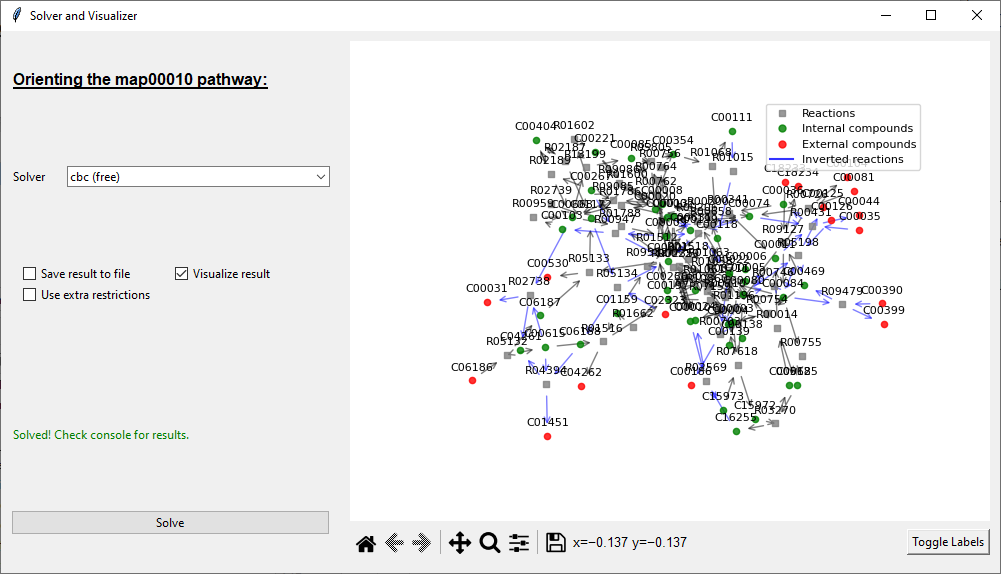
\includegraphics[width=0.8\textwidth]{Design of the User Interface/vis_labels.png}
    \caption{Solver-Visualizer - Visualizing a oriented pathway}
    \label{fig:vis_labels}
\end{figure}

In addition to the graphical representation, a Matplotlib-style toolbar is situated at the bottom right of the screen. This toolbar facilitates functionalities such as zooming in, moving the graph, and saving a screenshot of the graph. Furthermore, a dedicated button enables the toggling of labels on and off, enhancing visibility, especially in scenarios where nodes are densely clustered. The accompanying screenshot (Figure \ref{fig:vis_no_labels}) is the output of pressing the save button on the same pathway with improved visibility, achieved by activating the \textbf{Toggle Labels} button.

\begin{figure}[H]
    \centering
    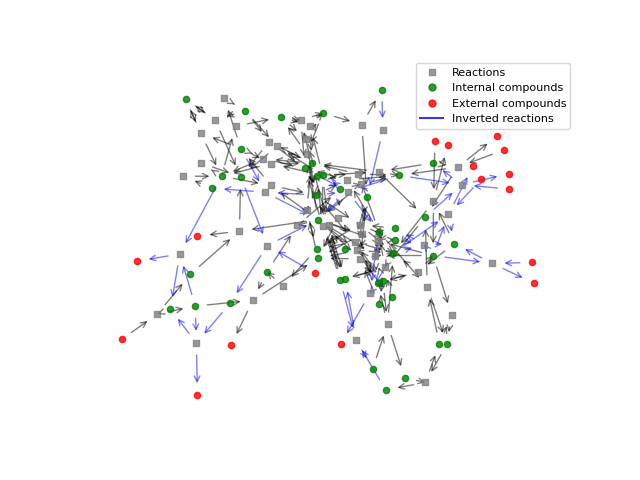
\includegraphics[width=0.8\textwidth]{Design of the User Interface/vis_no_labels.png}
    \caption{Solver-Visualizer - Visualizing a oriented pathway, with labels toggled off}
    \label{fig:vis_no_labels}
\end{figure}

Upon activating the \textbf{Use extra restrictions} tickbox, a new menu surfaces. This menu empowers the user to establish additional constraints, as elaborated in Section \ref{sec:extra_constraints} through to Section \ref{sec:extra_constraints_end}. Within this menu, users can prevent the inversion of specific reactions (or hyperedges), or classify particular compounds as external or internal. This feature provides a finer degree of control over the orientation and classification of elements in the hypergraph.

\begin{figure}[H]
    \centering
    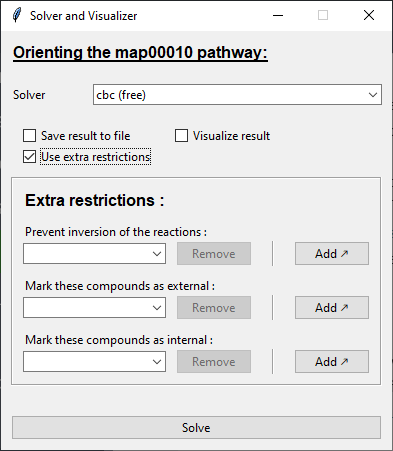
\includegraphics[width=0.6\linewidth]{Design of the User Interface/extra_constraints.png}
    \caption{Solver-Visualizer - The 'Extra restrictions' menu}
    \label{fig:enter-label}
\end{figure}

By default, each of the extra restriction fields begins empty.

To introduce a restriction, for example: preventing the inversion of reactions, users can click on the \textbf{Add} button. \\
This action triggers a popup window displaying a list of all potential values.\\In the case of our example, this list comprises reactions not yet marked as un-invertible. 

Following the popup invocation, users can select one or more items to incorporate into the restriction list. As demonstrated in Figure \ref{fig:extra_add}, an example showcases a user adding the reactions 'R00014', 'R00206', and 'R00341'.

\begin{figure}[H]
    \centering
    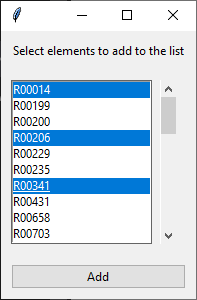
\includegraphics[width=0.35\linewidth]{Design of the User Interface/extra_add.png}
    \caption{Solver-Visualizer - Adding items to a list of a restriction}
    \label{fig:extra_add}
\end{figure}

Upon successful addition, the items are stored in the corresponding dropdown list. Figure \ref{fig:extra_success_add} illustrates the successful incorporation of items into the list.

\begin{figure}[H]
    \centering
    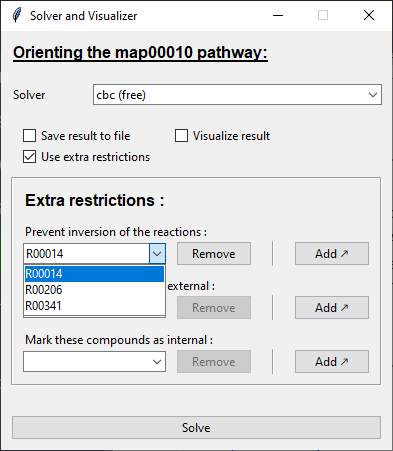
\includegraphics[width=0.5\linewidth]{Design of the User Interface/extra_success_add.png}
    \caption{Solver-Visualizer - Items added to a list of a restriction}
    \label{fig:extra_success_add}
\end{figure}

To remove an element from a restriction list, users can select the desired element from the corresponding dropdown menu and activate the \textbf{Remove} button. Figure \ref{fig:extra_remove} visually depicts the list after the user has pressed the \textbf{Remove} button, demonstrating the successful removal of an element from the restriction list.

\begin{figure}[H]
    \centering
    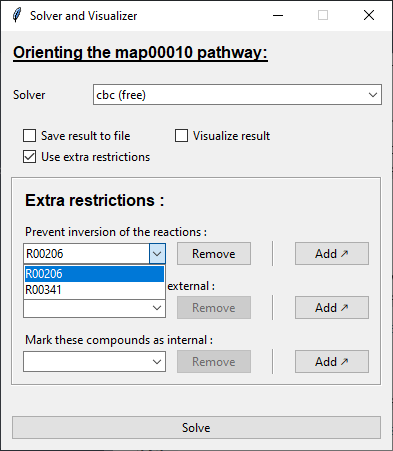
\includegraphics[width=0.5\linewidth]{Design of the User Interface/extra_remove.png}
    \caption{Solver-Visualizer - Item removed from a list of restrictions}
    \label{fig:extra_remove}
\end{figure}

During the optimization problem of orienting the pathway, we employ the AMPL model 'Model A' (refer to Section \ref{sec:model_a_b}), which, as demonstrated in Section \ref{sec:benchmark}, proves to be the most efficient model.

However, should the user opt for extra restrictions, we pivot to utilizing the model 'Serret DualImply extra restrictions' (refer to Section \ref{sec:model_dualimply_extra_restrictions}). As expounded in Section \ref{sec:math_proof}, this model is specifically designed to accommodate the additional constraints, as the mathematical robustness of the other model is insufficient for supporting these extra restrictions.

%%%%%%%%%%%%%%%%
%%%%%%%%%%%%%%%%

\subsection{Benchmark View} \label{sec:benchmark_view}

Upon initiating the "Benchmark View," users encounter a sleek and user-friendly interface, as showcased in Figure \ref{fig:benchmark-view}. Key components of this interface include a dropdown menu, enabling users to choose from solvers such as CBC, Gurobi, or CPLEX, and a prominent "Start Benchmark" button. The purpose of this thoughtful design is to simplify the benchmarking process, ensuring a seamless experience for users evaluating solver performance across a spectrum of optimization scenarios.

\begin{figure} [H]
\centering
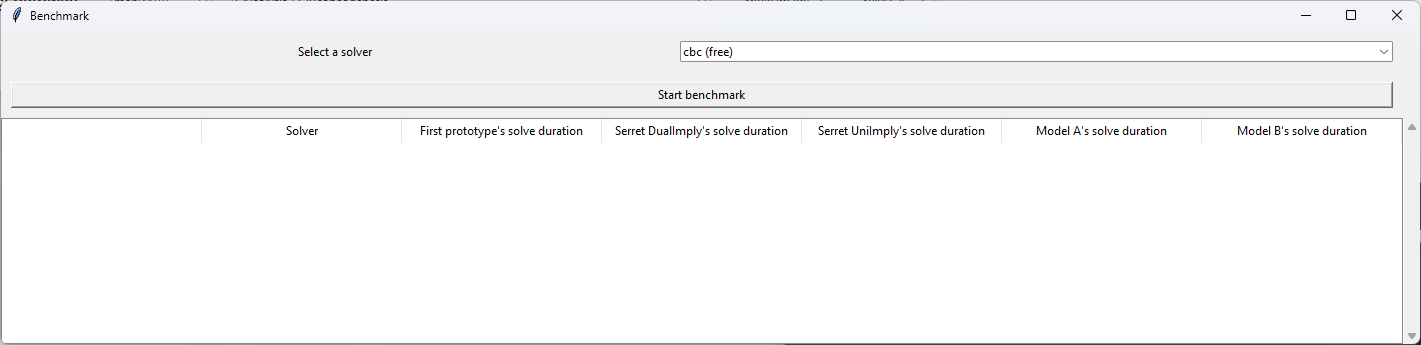
\includegraphics[width=0.8\linewidth]{Design of the User Interface/benchmark_View.png}
\caption{Benchmark View - User Interface}
\label{fig:benchmark-view}
\end{figure}

Upon triggering the "Start Benchmark" button, the benchmarking procedure commences. Each model, namely 'Model A,' 'Model B,' 'Serret Old,' 'Serret UniImply,' and 'Serret DualImply,' undergoes 25 optimizations. Subsequently, the results are presented in a Tk.TreeView below, offering users a comprehensive overview of solver performance across various models and optimizations.

The benchmarking process may take up to 4 minutes. Figure \ref{fig:benchmark-2-completed} illustrates the view after the completion of 2 benchmarks, each providing information on the date and time of completion, the utilized solver, and the average time taken by each model to solve individual optimization problems.

\begin{figure} [H]
\centering
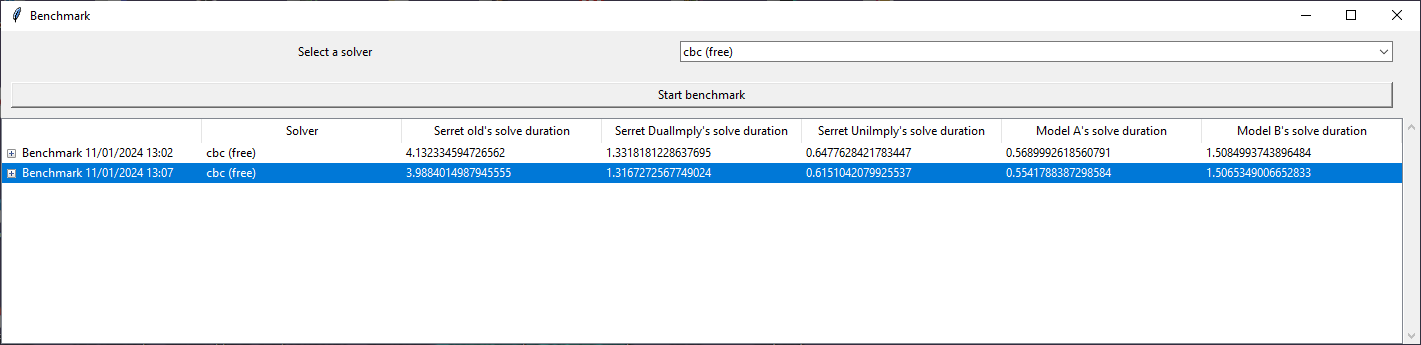
\includegraphics[width=0.75\linewidth]{Design of the User Interface/benchmark_2_completed.png}
\caption{Benchmark View - Completed Benchmarks}
\label{fig:benchmark-2-completed}
\end{figure}

For a more detailed analysis, users have the option to expand the benchmark report and delve into the completion details of each of the 25 entries, as demonstrated in Figure \ref{fig:expanded_benchmark}.

\begin{figure} [H]
\centering
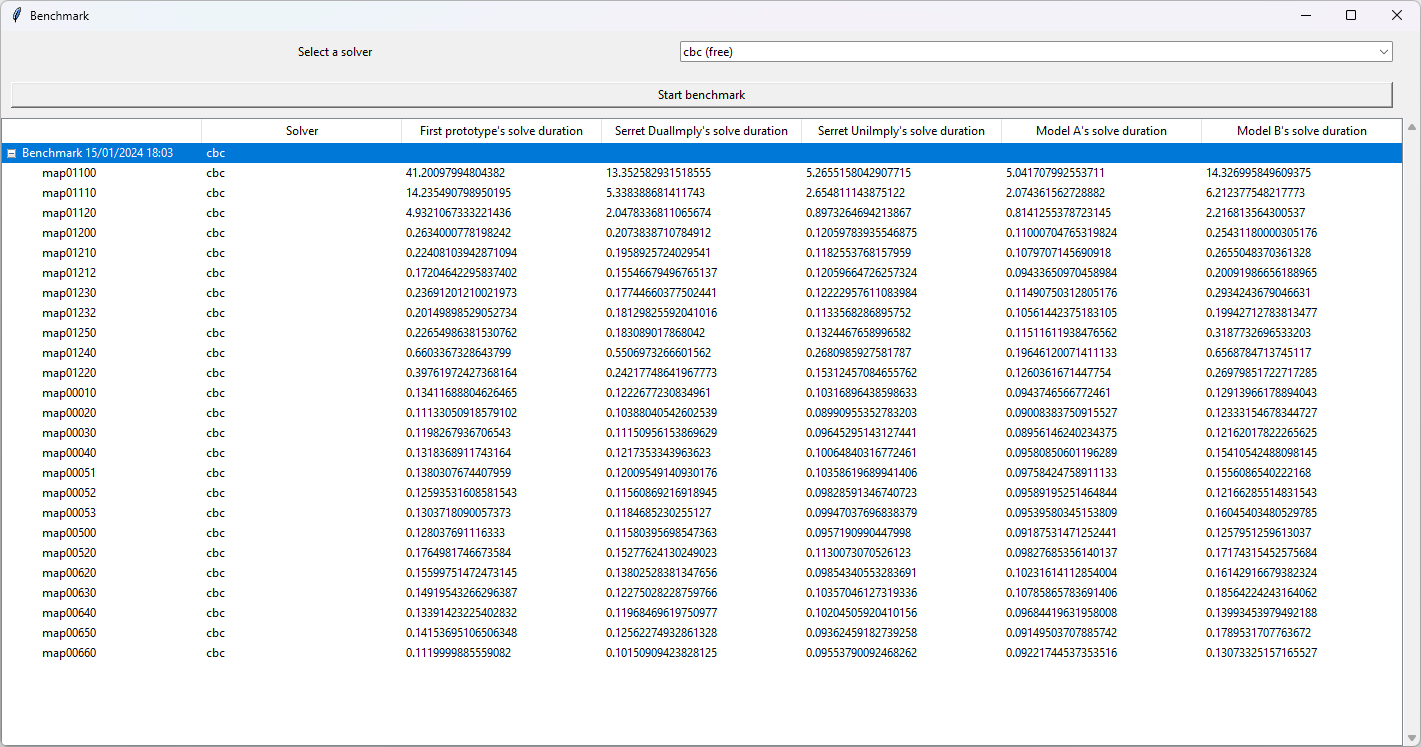
\includegraphics[width=0.75\linewidth]{benchmark_expanded.png}
\caption{Benchmark View - Expanded Benchmarks}
\label{fig:expanded_benchmark}
\end{figure}